%%% Conclusion
%%%%%%% Wording: ⏳
%%%%%%% Styling: ⏳
%%%%%%% References: ✅
%%%%% Grammar: ✅
%%% --------------------------------------------------------------
\chapter{Conclusion}
\label{ch:conclusion}


\begin{section}{Summary of Work}
	\label{sec:conclusion-summary}

	This thesis has been built upon two main pillars: \textbf{the analysis of the data collected by NFCtron's system} and \textbf{the development of an interactive dashboard} to visualize the findings.

	The analysis process started with the definition of the main research questions in cooperation with~\theOrganizer, resulting in a total of~\textbf{29 questions} to be answered.
	These questions were from a wide range of topics covering overall cashflow and revenue sources, system's performance, beverage consumption and customer behavior.
	A complete list of the research questions, together with the goals of the analysis, is covered in the~\fullref{ch:introduction}~chapter.

	Before conducting the analysis, exploration of the data, followed by the identification of the main data quality issues and the data cleaning process, was necessary.
	This process covered also the local environment setup, the data import process, and the data model of the system, all thoroughly described in~\autoref{ch:data-methodology}.
	Followed by a simple data anonymization process, the data was ready for the analysis.

	The main part of the thesis, the data analysis itself, resulted in the most voluminous part of the thesis – that being~\autoref{ch:data-analysis-and-results}.
	It was divided into the four research areas:~\fullref{sec:analysis-cashflow-and-revenue-sources},~\fullref{sec:analysis-performance-indicators},~\fullref{sec:analysis-beverage-consumption}, and~\fullref{sec:analysis-customers}.
	Each of these sections contained a detailed analysis of the data, answering the research questions in detail, presenting the findings in rich charts, diagrams, and tables, providing the required insights.

	The final part of the thesis, development of the interactive dashboard, was based on the findings of the analysis.
	This process took significant time and effort but resulted in an interactive dashboard that visualizes the most important findings of the analysis.
	Unfortunately, due to the time constraints, the dashboard was not fully completed, and some of the planned features were not implemented.
	The overall process of the implementation, from the initial approach, through core architecture, technical challenges faced, to the final implementation results and presentation of the dashboard, is described in~\autoref{ch:dashboard-implementation}.

	The thesis now concludes with the reflections on the project, the professional impact and outcomes, and the future impact of the thesis on the NFCtron Hub system, as well as the final thoughts on the project.
\end{section}

\begin{section}{Reflections}
	\label{sec:conclusion-reflections}

	Working directly with festival data revealed both challenges and opportunities that may impact future development in the NFCtron system.

	From a data perspective, the analysis revealed several opportunities for improving data collection.
	The need to manually add beverage volume information highlighted a gap in the current system's data model, which can unlock great insights with minimal effort.
	Similarly, the value of combining transaction data with event scheduling information demonstrated the importance of comprehensive data integration for meaningful insights.

	The necessity of data anonymization for privacy reasons highlighted the importance of data protection and possible future challenges in this area.
	However, a simple data anonymization process was enough for the current analysis, and the data was successfully anonymized without losing its analytical value, providing a lesson for future data handling.

	From the analytical side, the analysis process revealed the importance of defining clear research questions and objectives before starting the analysis.
	Initially, without having clear research questions, the analysis process was challenging, ineffective, and unstructured.
	However, this unstructured exploration phase was necessary to understand the data and to prepare multiple processes for the later data inspection.
	It also taught us various SQL techniques and optimization methods, from which we benefited in the later stages of the analysis and surely will benefit in the future.

	After defining specific research questions, the analysis process became more focused, efficient, and productive, leading to straightforward insights and findings.
	The presentation of the results was crucial for this analysis, but initially the data presentation was not optimal as preparing the data for the visualization is a meticulous process.
	If not done correctly, the results may be misleading or incorrect.
	However, with the right tools, techniques, and adequate presentations, the results can be easily understood and interpreted.
	Thanks to the necessity to present data in a clear and understandable way, various better visualization charts were learned and used in the analysis.
	This included charts such as the waterfall chart, packed bubble chart or a simple pie chart alternative – the waffle chart.

	Finally, the development of the interactive dashboard was a challenging but rewarding process, and the technical challenges faced provided valuable lessons.
	While the initial impulse often was to implement complex~\enquote{proper}~solutions, simpler approaches frequently proved to be more effective and efficient.
	This was particularly obvious in the caching system evolution, where a straightforward file-based solution ultimately outperformed more sophisticated alternatives for development purposes.

	Many situations require a balance between the complexity of the solution and the time available for implementation.
	As a result, the dashboard was not fully completed, and some of the planned features were not implemented, which leaves room for future development and improvements.

	Overall, the thesis provided required insights into the data, the analysis process, and the development of interactive dashboards.
	It showed the importance of clear research questions, data quality and processing and an understandable data presentation for effective analysis results.
\end{section}

\begin{section}{Professional Impact and Outcomes}
	\label{sec:future-impact}

	The main personal motivation for this thesis was to learn more about the data and demonstrate the findings in an interactive way, leading to more insights and knowledge for future updates of the NFCtron Hub dashboard.

	The research and analysis process has already given new understanding and knowledge about the data, the SQL techniques, and optimization methods.
	Thanks to this, we were already able to manage and deliver, together with our team, two significant updates to NFCtron Hub's analytical capabilities in late 2024.

	These updates resulted in a new time-based charts for ticket sales breakdowns and a comprehensive timeline view of festival activities, including its sales, refunds, customer arrivals, and customer ratings.
	A simple preview of this new timeline component can be seen in the~\autoref{fig:hub-chart-update} below.

	\begin{figure}[h]
		\centering
		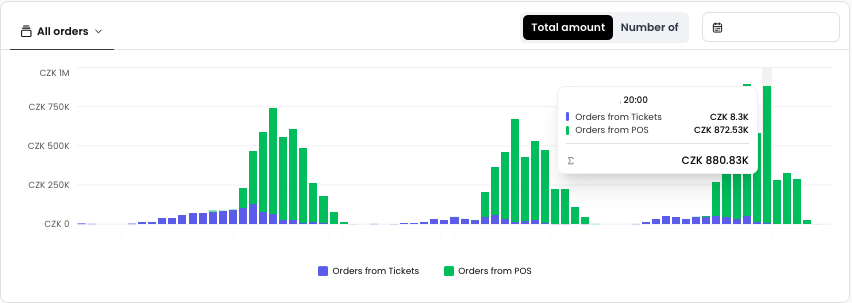
\includegraphics[width=\textwidth]{\ThesisFigures/ui/hub-chart-update}
		\caption{New Timeline Analysis in NFCtron Hub (December 2024 Update)}
		\label{fig:hub-chart-update}
		\source[NFCtron Hub\cite{nfctron_hub_nfctron_com}]
	\end{figure}

	Also, thanks to the analytical findings and problems encountered during the analysis, we were able to provide valuable feedback to the development team.
	This will lead to improvements in the data collection process and the data model of the system, which will make future analysis easier and more efficient.

	Finally, the knowledge acquired by this thesis still shapes our product development and enables us to provide more advanced analytical capabilities to our clients – festival organizers.
	Future development will build upon these foundations, further expanding the analytical capabilities of NFCtron's system.
\end{section}